% !TEX encoding = UTF-8 Unicode
%!TEX root = main.tex
% !TEX spellcheck = en-US
%%=========================================


%%%%%%%%%%%%%%%%%%%%%%%%%%%%%%%%%%%%%%%%%%%%%%%%%%%%%%%%%%%%%%%%%%%%%%%%%%%%%%%%%%%
\chapter{Design and Implementation}
\label{ch:design_implementation}
% each feature/

This chapter describes in detail the design and implementation of ProXC++. This includes the runtime data structures used by the scheduler, and how the library features interact with the scheduler and the runtime environment.

Note that the focus of this design and implementation is dynamic multithreading and multicore support. Features and details that has not much relevance to multithreading, such as replicators and C++ syntax, is detailed to a lesser extent.

The library is written in C++, with standard C++14 dialect. The reader is expected to have a fair understanding of C++, and being familiar with standard C++11 dialect or newer is recommended. Detailed explanations of the C++ programming language is not presented here. Refer to any C++ reference (e.g. \citet{stroustrup2013c++}) for more details.


\FloatBarrier
%%%%%%%%%%%%%%%%%%%%%%%%%%%%%%%%%%%%%%%%%%%%%%%%%%%%%%%%%%%%%%%%%%%%%%%%%%%%%%%%
\section{Data Structures}
% intrusive containers
% concurrent queues
% spinlocks


A set of data structures is commonly used by the runtime system. Apart from the C++ Standard Template Library (STL), the most notable data structures are \textit{intrusive containers}, \textit{concurrent queues}, and \textit{mutual exclusion locks}.

Intrusive containers, just as any other containers, stores some kind of data in some sort of way. The difference is how the container stores the necessary data used to organize the data. A non\hyp{}intrusive container is responsible for storing the necessary data, while for an intrusive container the elements are responsible for storing the necessary data. In other words, the element becomes ``aware'' of being a part of the intrusive container. Usually, intrusive containers are implemented with the elements having \textit{hooks} as data members. These hooks contains all the necessary data used by the intrusive container to store the elements. Intrusive containers offers better performance compared to non\hyp{}intrusive containers, as they minimize memory allocations and better memory locality.

Concurrent queues are queues which are safe to use concurrently, often denoted as \textit{thread safe}. The most common approach is taking a non\hyp{}thread safe queue and enforcing mutual exclusion around the critical regions. This approach however is not desirable, as it has very low throughput in multiprogrammed programs. Plenty of research \citep[e.g.][]{chase2005dynamic,le2013correct} has been devoted to creating non\hyp{}blocking queues (see \cref{sec:nonblocking_algorithms}) both available and efficient. Concurrent queues often differentiate between single or multiple producers and consumers. Producers are processes which insert elements into the queue, and consumers are processes which remove elements from the queue. The runtime system uses the variants \textit{single\hyp{}producer\hyp{}multiple\hyp{}consumer} (SPMC) queues and \textit{multiple\hyp{}producer\hyp{}single\hyp{}consumer} (MPSC) queues.

Creating a complete non\hyp{}blocking system is most of the times impossible for a multiprogrammed programs. Sometimes resorting to mutual exclusion in critical regions is unavoidable. Different types of locks is suitable for different situations. Whether the lock is often contested, meaning multiple kernel\hyp{}threads are trying to acquire the lock simultaneously, and if the lock is held for a longer period of time or not, will affect the performance. \Citet[page 196--199]{brown2007c++csp2} performs a case study on different mutexes, describing various mutex algorithms and provides a benchmark and analysis of their performance. The conclusion from the case study is that for low contested, short\hyp{}term held mutexes, spinlocks yields best performance regarding low latency. 

For multiprocessor architectures, the \textit{test\hyp{}and\hyp{}test\hyp{}and\hyp{}set} (TTAS) spinlock is generally favorable as it causes less memory contention than the standard spinlock. Instead of constantly trying to test\hyp{}and\hyp{}set the lock, it waits until the lock appears free. Different variants of the TTAS spinlock includes constant/exponential backoff during contention and cache friendly atomic operations.


\FloatBarrier
%%%%%%%%%%%%%%%%%%%%%%%%%%%%%%%%%%%%%%%%%%%%%%%%%%%%%%%%%%%%%%%%%%%%%%%%%%%%%%%%
\section{Runtime System Overview}
\label{sec:runtime_system_overview}

The runtime system for ProXC++ is based on \textit{contexts}, which represent a point of computational execution. A context is a user\hyp{}thread, meaning it has its own program stack and processor context. A kernel\hyp{}thread always has a main context and a scheduler context, while it may have zero or more work contexts. Contexts are based on the hybrid threading model (see \cref{subsec:threading_models}).

At startup, the initial main context creates $N-1$ kernel\hyp{}threads, given the processor has $N$ online logical cores. Each main context then creates a scheduler context, which represent the runtime environment for each kernel\hyp{}thread. Only the initial main context does any meaningful work, as the other main contexts only purpose is to spawn and join the scheduler context. Whenever the initial main context returns, the runtime environment will cleanup and shutdown. At the creation of a new kernel\hyp{}thread, along side with its main context and scheduler context, the scheduler will wait as idle (block) until available work is ready in other schedulers.

\Cref{fig:runtime_overview} displays a rough outline of how the contexts, user\hyp{}threads and kernel\hyp{}threads are organized relative to each other. Note that even though work contexts are present in each kernel\hyp{}thread, it 

\begin{figure}[h!]
    \centering
    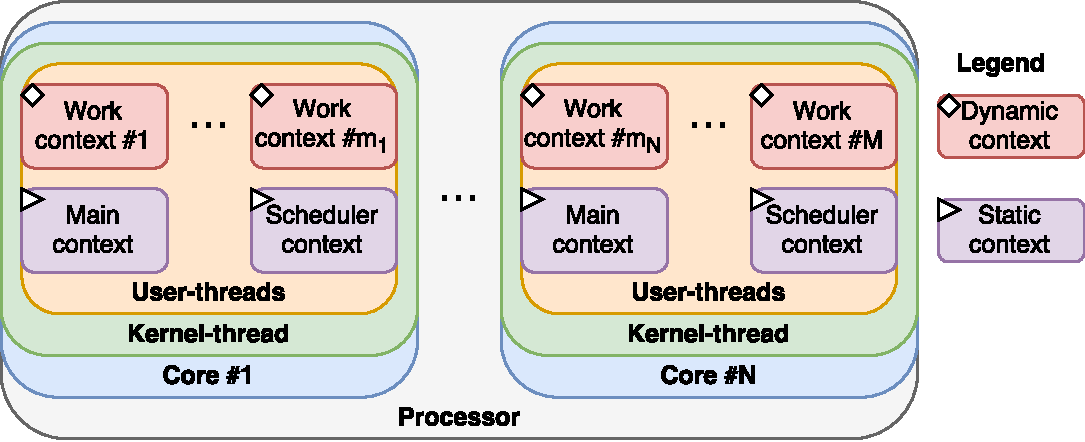
\includegraphics[width=0.8\linewidth]{fig/runtime_overview}
    \caption{Overview of the runtime system, with N online processor cores.}
    \label{fig:runtime_overview}
\end{figure}

Work is distributed among schedulers through work stealing (see \cref{subsec:work_stealing}). This is achieved by each scheduler having a double\hyp{}ended queue (deque for short) containing ready work for that given scheduler. Whenever work is spawned by a scheduler, or idle work becomes ready, it is pushed onto the deque. This allows idle schedulers to try steal work and resume.


\FloatBarrier
%%%%%%%%%%%%%%%%%%%%%%%%%%%%%%%%%%%%%%%%%%%%%%%%%%%%%%%%%%%%%%%%%%%%%%%%%%%%%%%%
\subsection{Contexts}
\label{subsec:contexts}

The runtime system differentiates contexts in two categories: \textit{process vs. scheduler} and \textit{static vs. dynamic}.

A process context represents a part of computation from the program, while the scheduler context is, as the name implies, the scheduler which is in control of scheduling the different process contexts. A static context is a context which cannot \textit{migrate} between schedulers, while a dynamic context can.

For every kernel\hyp{}thread, there always exist a \textit{main context} and a \textit{scheduler context}. The main context is the context of the actual kernel\hyp{}thread, meaning the kernel\hyp{}thread returns when the main context returns. It is a process context, since it represents a part of the computation in the program, and a static context, since it cannot migrate between schedulers. It is undefined behaviour FIXME for main context to return (exit) on a kernel\hyp{}thread different from where it originated from, which is why the main context is static.

The scheduler context is responsible for creating new work contexts, schedule between work contexts, and destroying finished work contexts. The scheduler is never visible to the programmer, and is the driving force behind the runtime environment. The scheduler is obviously a static context, as having multiple schedulers on the same kernel\hyp{}thread is unintuitive and unproductive.

Besides the main and scheduler context, the rest of the program is composed by \textit{work contexts}. Work contexts are process contexts, but opposed to the main context, are dynamic instead of static. Being dynamic allows work contexts to migrate between schedulers. 

Contexts are implemented using the Boost Context library \citep{kowalke2017boost}. Boost Context creates an abstraction over the execution state of a thread called \textit{execution context}, which includes stack and stack pointer, local variables, CPU registers and flags, and instruction pointer. The execution context allows transfer of control between other execution contexts, allowing to build higher level abstractions such as user\hyp{}threads. Execution contexts can also migrate between kernel\hyp{}threads.

The context data structure is represented as a class, containing an execution context as well as a collection of flags, intrusive hooks, a wait queue, and a spinlock. The context class only acts as an information container for a given user\hyp{}thread, as most of the functionality of the context is implemented by the scheduler.

\begin{figure}[h!]
    \centering
    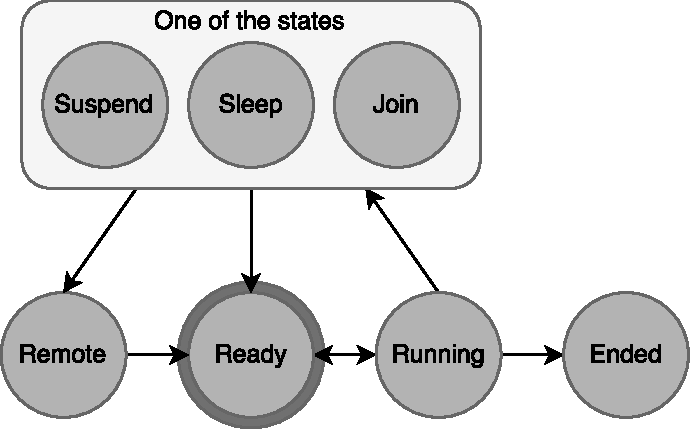
\includegraphics[width=0.6\linewidth]{fig/context_states}
    \caption{Finite state machine of context states and transitions.}
    \label{fig:runtime_overview}
\end{figure}


\FloatBarrier
%%%%%%%%%%%%%%%%%%%%%%%%%%%%%%%%%%%%%%%%%%%%%%%%%%%%%%%%%%%%%%%%%%%%%%%%%%%%%%%%
\subsection{Processes}
\label{subsec:processes}

A concurrent program using ProXC++ consists of \textit{processes}, called \textit{proc} in code. These processes, same as in CSP, are independent points of execution, with each running sequential code. In code, a process is represented by a function and its corresponding arguments. When scheduled, the function is executed concurrently with the rest of the program, and exits when the function returns. 

The process is no more than an opaque type to a context. The programmer implicitly creates new contexts through processes, while the scheduler under the hood operates on the contexts.

Processes can be dynamically generated, either through explicitly creating a dynamic collection of processes or through use of replicators.

% Talk more about single processes and replicated processes, how they are defiend, how they work etc.


\FloatBarrier
%%%%%%%%%%%%%%%%%%%%%%%%%%%%%%%%%%%%%%%%%%%%%%%%%%%%%%%%%%%%%%%%%%%%%%%%%%%%%%%%
\subsection{Scheduler}
\label{subsec:scheduler}
% work stealing
% process create, schedule, join, destroy
% process timeouts

The scheduler is the corner piece of runtime system. It has the sole responsibility of managing the different contexts, including creating, scheduling, and destroying contexts. The scheduler runs as its own context, running in an scheduler loop until the program exits. Each spawned kernel\hyp{}thread contains a scheduler context, and the scheduler context never migrates to an another kernel\hyp{}thread. Each scheduler is the ``owner'' of one or more process contexts. ``Owning'' a context is synonymous with management; scheduling, inter\hyp{}process handling, and destroying the context when the corresponding process terminates. When a process is created, the scheduler residing on the same kernel\hyp{}thread ``owns'' that context. Only one scheduler can ``own'' a context at a time.

A scheduler consists of context queues, scheduler functionality, and a scheduler context running an event loop.


\FloatBarrier
%%%%%%%%%%%%%%%%%%%%%%%%%%%%%%%%%%%%%%%%
\subsubsection{Context Queues}

Each scheduler has five queues: \textit{ready}, \textit{work}, \textit{sleep}, \textit{terminated}, and \textit{remote} queue. The ready queue holds the set of contexts ready to be scheduled, and is explained in more detail later. The work, sleep and terminated queue is managed only by a single scheduler, and is used to organize the processes the scheduler ``owns''. The work and terminated queues are intrusive doubly linked lists, while the sleep queue is a sorted, intrusive multiset\footnote{A multiset is an associative container that contains a set of objects, which allows multiple keys with the same values.}. The work queue is the total list of all processes the scheduler ``own''. The sleep queue contains all process which are suspended with a given timeout, and are sorted in ascending order. The terminated queue is the queue of all processes which has terminated. The need for this queue will be explained later. 

The remote queue is a concurrent MPSC queue, where the managing scheduler is the consumer while any other schedulers are the producers. Whenever a scheduler readies a context and it does not ``own'' it, the context is placed in the remote queue to the ``owning'' scheduler. The ``owning'' scheduler transitions contexts in the remote queue to the ready queue. In essence, the remote queue is used to signal schedulers when their contexts are readied, since remote schedulers cannot safely access the ready queue.

Now, back to the ready queue. The ready queue, as mentioned above, contains all contexts ready to be scheduled for a given scheduler. Only contexts the scheduler ``owns'' can be enlisted to the ready queue. From the schedulers point of view, the ready queue is a black box. Readied contexts are enqueued to the ready queue, and ready contexts are dequeued when scheduling a new context. How the contexts are stored internally and the policy of what order the contexts are dequeued is determined by the \textit{scheduling policy}. The default scheduling policy in ProXC++ is work stealing, however any other kind of policy could be implemented, such as work sharing and round robin.

The work stealing scheduling policy is implemented as a concurrent double\hyp{}ended SPMC queue, using the design presented in \citet{chase2005dynamic,le2013correct} for efficient non\hyp{}blocking work stealing. The managing scheduler is the producer, while all schedulers are the consumers. The ready queue is responsible for load balancing work between the schedulers. From a schedulers point of view, it cannot tell if a dequeued ready context was stolen or not. It also cannot tell if other ready queues steals from its own ready queue. 


\FloatBarrier
%%%%%%%%%%%%%%%%%%%%%%%%%%%%%%%%%%%%%%%%
\subsubsection{Scheduler Functionality}
% framework
% context switch data
% context launch
% context joining
% context wait
% context 

Maybe the most important part of the scheduler is context management. The scheduler is responsible for creating new and destroying finished contexts, and 


\FloatBarrier
%%%%%%%%%%%%%%%%%%%%%%%%%%%%%%%%%%%%%%%%
\subsubsection{Scheduler Event Loop}

The scheduler event loop is the where the entirety of the scheduler context's lifetime executes in. The event loop consists of the following: check of exit flag, context cleanup, context transitions, and context scheduling. See \cref{lst:scheduler_event_loop} for pseudo code reference.

\begin{lstfloat}
\begin{lstlisting}[caption={Scheduler event loop pseudo code.}, label={lst:scheduler_event_loop}, style={CustomC}, xleftmargin={4em}]
void scheduler_event_loop() {
    while ( true ) {
        // check exit flag and break if all workers have finished
        if ( exit_flag ) {
            scheduling_policy.notify();
            if ( work_queue.empty() ) {
                break;
            }
        }
        // cleanup terminated contexts
        cleanup_terminated();
        // transition contexts to ready
        transition_remote(); // remote -> ready
        wakeup_sleep();      // sleep  -> ready
        // schedule ready context if any else wait
        context = scheduling_policy.dequeue();
        if ( context != nullptr ) {
            // scheduler must always be available
            scheduling_policy.enqueue( scheduler_context );
            // context switch to ready context
            resume( context );
            // scheduler is now running
        } else {
            // sleep until first sleeping context timeout
            // or wait until notified
            time_point = ( sleep_queue.empty() )
                ? time_point_max
                : sleep_queue.first() ;
            scheduling_policy.suspend_until( time_point );
        }
    }
    // scheduler is exiting, cleanup scheduler
    scheduler_cleanup();
    // lastly, context switch to main
    resume( main_context );
}
\end{lstlisting}
\end{lstfloat}





\FloatBarrier
%%%%%%%%%%%%%%%%%%%%%%%%%%%%%%%%%%%%%%%%%%%%%%%%%%%%%%%%%%%%%%%%%%%%%%%%%%%%%%%%
\section{Parallel Statement}
\label{sec:parallel_statement}

Processes can spawn new processes in parallel with the \textit{parallel} statement. The parallel statement takes one or more processes, either as single process statements or process replicators, and spawns and runs these processes in parallel. The spawned processes runs concurrently with any other processes currently running in the program. The parallel statement is the only way to spawn new processes with ProXC++.

The parallel statement follows the fork\hyp{}join model \citep[page 88]{mccool2012structured}, where a sequential execution branches off at a designated point into parallel work, and subsequently joins/merges at another designated point and resumes the original sequential execution. \Cref{fig:fork_join_model} gives a simple illustration of the fork\hyp{}join model.

\begin{figure}[h!]
    \centering
    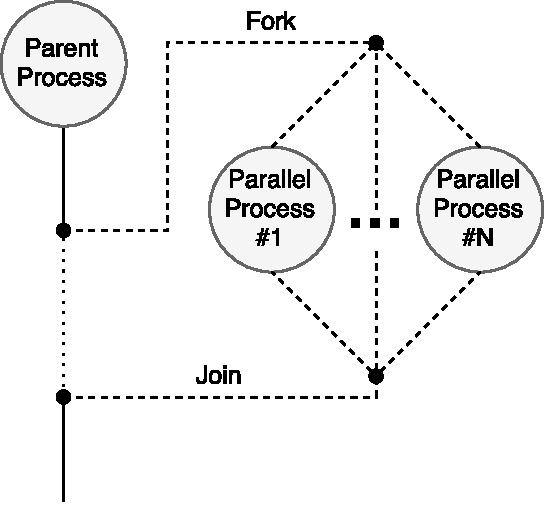
\includegraphics[width=0.6\linewidth]{fig/fork_join}
    \caption{A parent process spawns $N$ parallel processes following the fork\hyp{}join model.}
    \label{fig:fork_join_model}
\end{figure}

The process calling the parallel statement is the parent process. When calling the parallel statement, the parent process is suspended until all processes within the parallel statement has spawned, executed and terminated. When all parallel processes has terminated, the parent process resumes execution. 

The processes to be executed in parallel can be defined in two ways: either as a single process or as a replicated process. See \cref{subsec:processes} for a more detailed explanation of processes. 


\FloatBarrier
%%%%%%%%%%%%%%%%%%%%%%%%%%%%%%%%%%%%%%%%
\subsection{Parallel Implementation}
\label{subsec:parallel_implementation}

All relevant code for the parallel statement implementation can be found in the following files \texttt{parallel.hpp} and \texttt{process.hpp}.

The parallel statement has two obvious phases: the fork and join phases. 

During the fork phase, each process to be executed in parallel is spawned by the parent process, one by one. This involves creating the process, attaching the process to the current scheduler, and launching the process. Launching the process simply enqueues the process to the ready queue of the current scheduler. When all parallel process has been spawned, the parent process enters the join phase.

The join phase consists of the parent process joining all parallel processes, one by one. Joining a process, which is an atomic operation, involves waiting until the process has terminated. One of two things happen when joining: either the process has not terminated and is still executing, or it has terminated. If the process has terminated, the parent process continues the join phase. If not, the parent process waits. When the process terminates, it will wake up the parent process.

Pseudo code for the parallel implementation is presented in \cref{lst:parallel_statement_pseudo_code}.

\begin{lstfloat}
\begin{lstlisting}[caption={Parallel statement pseudo code.}, label={lst:parallel_statement_pseudo_code}, style={CustomC++}, xleftmargin={4em}]
/* fork phase */
for_each process in parallel_processes {
    process.fork();
}
/* join phase */
for_each process in parallel_processes {
    process.join();
}
\end{lstlisting}
\end{lstfloat}

The parallel statement is quite simplistic, as it only enqueues new processes to the current scheduler and waits for their termination. Much of the simplicity comes from the lack of a \textit{sequential} statement, simplifying the design significantly. 


\FloatBarrier
%%%%%%%%%%%%%%%%%%%%%%%%%%%%%%%%%%%%%%%%%%%%%%%%%%%%%%%%%%%%%%%%%%%%%%%%%%%%%%%%
\section{Timers}
\label{sec:timers}

Three types of timers are available: \textit{egg}, \textit{repeat} and \textit{date} timer. Timers are used for either explicit process suspension, or for timeout on channel or alternation operations. 

Egg timer is used for relative timeout. Just as an egg timer in real life, it is used to countdown for a specified period of time. It is not a one\hyp{}shot timer, meaning the same timer can be reused multiple times. The countdown begins at the start of an operation, effectively resetting the timer if already used.

Repeat (or loop) timer is used for a periodic repeating timeout. The repeat timer will timeout in a periodic fashion, given a specified period of time. The timer only resets after timeout. Compared to the egg timer, the repeat timer is also not a one\hyp{}shot timer and can be reused, but the repeat timer does not reset the countdown at the start of an operation.

Date timer is used for absolute timeout. It is a one\hyp{}shot timer, and will always be expired after timeout. The date timer timeouts at a specified time point. The timer can never be reset, and therefore survives multiple operations.


\FloatBarrier
%%%%%%%%%%%%%%%%%%%%%%%%%%%%%%%%%%%%%%%%
\subsection{Timer implementation}
\label{subsec:timer_implementation}

All relevant code for the timer implementation can be found in the following file \texttt{timer.hpp}.

Timers are represented through a common abstract class interface, shown in \cref{lst:timer_class_interface}. Instances of an egg or repeat timer converts the specified time duration to a time point, while the date timer already specifies a time point. This time point is stored in the base interface class. All timers support duration and time points from the standard library \texttt{std::chrono}.

\begin{lstfloat}
\begin{lstlisting}[caption={Timer class interface.}, label={lst:timer_class_interface}, style={CustomC++}, xleftmargin={4em}]
class timer::Interface {
protected:
    using TimePointT = /* implementation defined */;
    TimePointT time_point_;
public:
    virtual void reset() = 0;
    virtual bool expired() = 0;
    bool operator<( Interface const & other ) const 
    { return time_point_ < other.time_point_; }
    TimePointT const & get() const { return time_point_; }
};
\end{lstlisting}
\end{lstfloat}

When a timer is supplied for a timed operation, the reset method is called. For the egg timer, a reset results in calculating new time point. For the repeat timer, the next periodic time point is calculated if expired, else the time point remains the same.

For some operations, such as alternation, multiple timers can be supplied. Since timers have a static time point after reset, the closest time point is chosen for timeout.

Under the hood, an explicit process suspension with a given timer is simply enlisting the context to the scheduler sleep queue with the corresponding time point. When the time point is reached, the scheduler removes the context from the sleep queue and is rescheduled. The time point is checked by the scheduler context in the \texttt{wakeup\_sleep()} method. If the time point has already reached when suspending the process, it immediately returns. 

A timed operation differs slightly. Whenever the context waits for some event during the operation, the context is enlisted in the scheduler sleep queue. Now, one of two things may happen: either the context is rescheduled by some event, or the operation times out and is rescheduled by the scheduler. If the context was rescheduled by the event, the scheduler removes the context from the sleep queue and is enqueued in the ready queue. If the time point expires, the scheduler transitions the context from the sleep queue to the ready queue in the \texttt{wakeup\_sleep()} procedure. Either way, the context is removed from the sleep queue and enqueued in the ready queue.

Note that if the context is rescheduled by a remote event, the context is enlisted in the remote queue first, but it is not removed from the sleep queue. Its not until the scheduler transitions the context from remote to ready during the \texttt{transition\_remote()} procedure the context is removed from the sleep queue.


\FloatBarrier
%%%%%%%%%%%%%%%%%%%%%%%%%%%%%%%%%%%%%%%%%%%%%%%%%%%%%%%%%%%%%%%%%%%%%%%%%%%%%%%%
\section{Channels}
\label{sec:channels}

Channels forms the only means of communication as well as synchronization between processes via message\hyp{}passing. Given a channel, some type of message can be transmitted between a sender and a receiver.

Hereafter, the term ``\textit{Tx}'' denotes a process sending on a channel, and the term ``\textit{Rx}'' denotes a process receiving on a channel. The term ``\textit{participant}'' denotes either a Tx or Rx.

An synchronous channel implies both a Tx and a Rx must be at the channel to complete the channel operation, e.g. a Tx cannot transmit a message without a Rx ready to receive. If only one of the two required participants are ready to transmit, the participant must block (wait) until the other side is ready. This kind of behaviour is called rendezvous. A synchronous channel is also unbuffered, given that no messages are stored intermediately in the channel.

The opposite of a synchronous, unbuffered channels are asynchronous, buffered channels, where messages are buffered if there are no receivers ready. Tx never waits regardless of a ready Rx or not, while Rx must only wait if the buffer is empty. See \cref{fig:channel_sync_async} for an illustration of the difference between a synchronous and asynchronous channel.

\begin{figure}[h!]
    \centering
    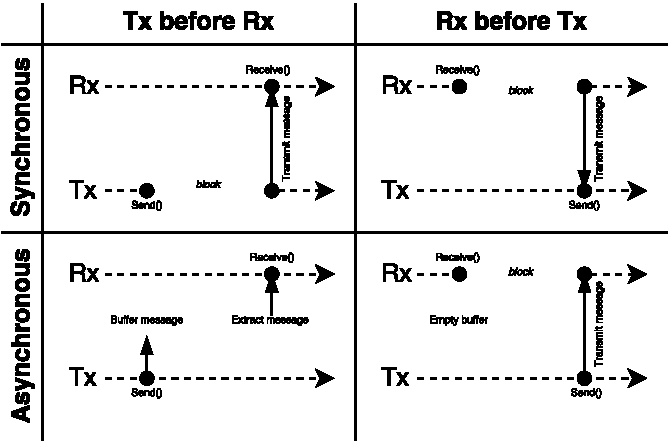
\includegraphics[width=0.9\linewidth]{fig/channel_sync_async}
    \caption{Different configurations of synchronous and asynchronous channel communication.}
    \label{fig:channel_sync_async}
\end{figure}

A unidirectional channel only allows messages to be transmitted in one direction. In contrast, a bidirectional channel allows messages to be transmitted in both directions.

Some channel design has the concept of limiting how many unique processes can access and use a channel. This concept is called \textit{disjointness rules} in XC \citep{douglas2009programming} and \textit{usage rules} in occam \citep{barrett1992occam}. In essence, these ``rules'' specify if either end of a channel, sending and receiving, can only be used by a unique process or any processes. Usually denoted by \textit{one/any\hyp{}to\hyp{}one/any}, this gives the four configurations: \textit{one\hyp{}to\hyp{}one}, \textit{one\hyp{}to\hyp{}any}, \textit{any\hyp{}to\hyp{}one}, and \textit{any\hyp{}to\hyp{}any}. Both XC and occam follows the one\hyp{}to\hyp{}one design.

Ensuring both Tx and Rx agrees on the type of message being transmitted has to do with \textit{type safety}. If both participants of a channel operations disagrees in the type of the transmitted message, a \textit{type error} occurs. Type safety is therefore to discourage or prevent type errors. It is obviously desirable for a type safe channel, but it is highly dependent on support from either the programming language or the compiler to enforce type safety. A compromise is size safe channels, where both participants agree on the size of the message rather than the type. Size safety is not as desirable as type safety, but is much more doable to enforce.


\FloatBarrier
%%%%%%%%%%%%%%%%%%%%%%%%%%%%%%%%%%%%%%%%
\subsection{Channel Algorithm}
\label{subsec:channel_algorithm}

The channel algorithm is different whether the channel end is alting or not. A set of conjectures is postulated in \cref{list:conjecture_both,list:conjecture_nonalting,list:conjecture_alting} to form the basis of the channel algorithm.

\FloatBarrier

\begin{enumeratefloat}
    \caption{Conjectures for both non\hyp{}alting and alting channel ends.}
    \label{list:conjecture_both}
    \begin{enumerate}[topsep=0em,itemsep=-1em,partopsep=0.5em,parsep=1em]
        \item A channel operation consists of a single Tx and a single Rx arriving in either sequential order, both of which can be alting or non\hyp{}alting.
        \item When a channel end has arrived for a channel operation, another channel end of same type cannot arrive before that channel operation has completed.
        \item Any channel end may at most suspend once during a channel operation.
        \item The last channel end to arrive at a channel operation will always complete the item transmission.
        \item If a channel end is suspended during a non\hyp{}timed channel operation, it is only rescheduled if the channel operation completed or the channel closed.
        \item During a timed channel operation, a suspended channel end may also be rescheduled if a timeout occurs.
    \end{enumerate}
\end{enumeratefloat}

\begin{enumeratefloat}
    \caption{Conjectures for non\hyp{}alting channel ends.}
    \label{list:conjecture_nonalting}
    \begin{enumerate}[topsep=0em,itemsep=-1em,partopsep=0.5em,parsep=1em]
        \item The non\hyp{}alting channel end arriving first at an channel operation will always suspend.
        \item The channel end arriving last at an channel operation will never suspend.
        \item A process holding both channel ends for a channel will always block indefinitely if operating on the given channel.
        \item A channel end never leaves the channel operation after arrival unless it completes, the channel closes, or times out, i.e. a channel end always commits to a channel operation.
    \end{enumerate}
\end{enumeratefloat}

\begin{enumeratefloat}
    \caption{Conjectures for alting channel ends.}
    \label{list:conjecture_alting}
    \begin{enumerate}[topsep=0em,itemsep=-1em,partopsep=0.5em,parsep=1em]
        \item A channel end never explicitly suspends during a channel operation. This is done indirectly by the alting procedure.
        \item A channel end may leave the channel operation after arrival and return later, i.e. a channel end may not commit to a channel operation.
    \end{enumerate}
\end{enumeratefloat}

\FloatBarrier

A key observation to make from the conjectures is the symmetry of a channel operation. It is invariant Tx or Rx is completing the operation. This makes the algorithm very much the same for both sending and receiving on a channel. Another observation to make is how non\hyp{}alting channel ends commit, while alting channel ends may not commit. This skew in committal channel ends allows for important assumptions in the algorithm.


%%%%%%%%%%%%%%%%%%%%%%%%%%%%%%%%%%%%%%%%
\subsubsection{Non\hyp{}Alting Channel End Algorithm}

A non\hyp{}alting channel end has two cases to consider: either the other channel end is non\hyp{}alting or alting. 
A channel operation for a non\hyp{}alting channel end can be considered to consists of three possible steps:

\begin{enumerate}[topsep=0em,itemsep=-1em,partopsep=0.5em,parsep=1em]
    \item \textbf{Check channel is open} -- return if the channel is closed, else continue.
    \item \textbf{Check for opposite channel end} -- if an opposite channel end is present at the channel, try selecting the channel end. If successful, complete the transmission, reschedule opposite channel end and return ok. Else, continue.
    \label{step:channel_nonalt_complete}
    \item \textbf{Wait for opposite channel end} -- register the channel end in the channel and suspend. When rescheduled, check if the item was transmitted or not and return appropriately.
    \label{step:channel_nonalt_wait}
\end{enumerate}

Note that the entire procedure is surrounded by mutual exclusion using the channel lock, because the channel ends must arrive at the channel in a sequential order.

To elaborate on step \ref{step:channel_nonalt_complete}, selecting the opposite channel end is necessary since an alting opposite channel end is not committal to the channel operation, even though it is present. Selecting a non\hyp{}alting channel end is always successful since it is always committal, while an alting channel end may fail. This selection process is further explained in \cref{sec:alternation_choice}.

Completing the transmission in step \ref{step:channel_nonalt_complete} involves transmitting the item and setting the consumed flag, and checking the transmission in step \ref{step:channel_nonalt_wait} involves checking and resetting the consumed flag.

The consumed flag is necessary to signal the suspended channel end if the item was transmitted, even though the channel has been closed. Consider this situation: Tx enters the channel and is suspended, waiting for an Rx. Rx enters the channel, completes the transmission, and reschedules Tx. Before Tx is resumes execution, Rx closes the channel. Now, when Tx resumes it is impossible to tell if Tx was rescheduled because of completed operation or channel closing. The consumed flag is here to signal the rescheduled channel end was rescheduled because of either case.


%%%%%%%%%%%%%%%%%%%%%%%%%%%%%%%%%%%%%%%%
\subsubsection{Alting Channel End Algorithm}

An alting channel end also has two cases to consider: either the other channel end is non\hyp{}alting or alting. The non\hyp{}alting case is trivial, because if the opposite end is present then simply complete the transmission. The alting case is however more complicated. 

Before describing the algorithm, first consider this situation: Two processes both alting on the same two channels, however each process have the Tx of one channel and Rx of the other, making a cycle. See \cref{fig:alting_problem} for illustration. Both of these alting processes must somehow agree on which case they both select. Some sort of synchronization between two alting channel ends must therefore exist. Note that this alt\hyp{}to\hyp{}alt synchronization must be asymmetrical to avoid deadlocks.

\begin{figure}[h!]
    \centering
    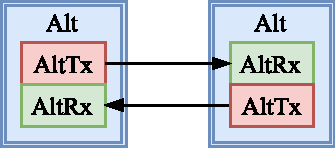
\includegraphics[width=0.6\linewidth]{fig/alting_problem}
    \caption{Illustration of the cyclic alting problem.}
    \label{fig:alting_problem}
\end{figure}

A value with three possible states is used for alt\hyp{}to\hyp{}alt synchronization. The three states are \textit{none}, \textit{offered}, and \textit{accepted}. Given all alting channel ends have a well defined static ordering, the alt\hyp{}to\hyp{}alt synchronization protocol says the lower ranked channel end is to offer synchronization, while the higher ranked channel end is to accept. Note that for this to not be symmetric, the ordering must be invariant of the channel end type.

Given this alt\hyp{}to\hyp{}alt synchronization, the alting channel end algorithm is as follows:

\begin{enumerate}[topsep=0em,itemsep=-1em,partopsep=0.5em,parsep=1em]
    \item \textbf{Check alt\hyp{}to\hyp{}alt synchronization} -- if an opposite channel end is present and is alting, check synchronization state. Else, continue. If offered, accept and complete the alt\hyp{}to\hyp{}alt transmission. Else, return and try later.
    \label{step:check_alt_sync}
    \item \textbf{Check channel is open} -- return if the channel is closed, else continue.
    \item \textbf{Check for opposite channel end} -- return if there is no opposite channel end present, else continue.
    \item \textbf{Check if opposite channel end is non\hyp{}alting} -- if the opposite channel is non\hyp{}alting, complete the transmission, reschedule opposite channel end and return ok. Else, continue.
    \label{step:opposite_side_nonalting}
    \item \textbf{Check rank of opposite channel end} -- compare the rank of the opposite channel end with self.
    \item \textbf{Self has lower rank} -- offer synchronization and wait until response. If the sync was accepted, return ok. Else, return appropriately.
    \label{step:self_lower_rank}
    \item \textbf{Self has higher rank} -- check synchronization state. If offered, complete transmission and accept synchronization. Else, return appropriately.
    \label{step:self_higher_rank}
\end{enumerate}

The reason for checking the alt\hyp{}to\hyp{}alt synchronization in step \ref{step:check_alt_sync} before checking the channel is open has to do with acquiring the channel lock. Since the lock is held by the opposite channel end while offering synchronization, an offered synchronization must be resolved before acquiring the channel lock.

In step \ref{step:opposite_side_nonalting} the alting channel end does not need to synchronize with the opposite channel end if it is non\hyp{}alting, due to selecting a non\hyp{}alting channel ends always succeeds. 

The synchronization procedure in step \ref{step:self_lower_rank} is a little more convoluted than stated, since the alt\hyp{}to\hyp{}alt synchronization is only needed if the opposite alting procedure is checking. If it is waiting, normal selection is used.

The synchronization procedure in step \ref{step:self_higher_rank} is more straightforward. If synchronization is offered, complete the transmission and accept. If it is not offered, check the alting procedure state. If the alting procedure state is checking, try later. If the state is waiting, try normal selection. 


\FloatBarrier
%%%%%%%%%%%%%%%%%%%%%%%%%%%%%%%%%%%%%%%%
\subsection{Channel Implementation}
\label{subsec:channel_implementation}

All relevant code for channel implementation is found in the file \texttt{channel.hpp} and all files within the folder \texttt{channel/}.

In ProXC++, channels exist in one flavour: synchronous and unbuffered, unidirectional, one\hyp{}to\hyp{}one, and type safe. All channel related objects and methods reside in the \texttt{channel} namespace.

Channels are composed of the two channel end objects \texttt{Tx<T>} and \texttt{Rx<T>}. \texttt{Tx<T>} and \texttt{Rx<T>} can send and receive on a channel, respectively. Channels can only be created through the functions \texttt{create<T>()} for single channel objects, or \texttt{create\_n<T>()} for $n$ channel objects, \cref{lst:channel_create_functions} for reference. 

Channel operations, alting or not, can be timed with a timer. Both sending and receiving channel ends can be used in alternation, compared to occam and XC which only permits receiving channel ends.

Channels can be closed. When a channel is closed, no more channel operations can be completed on the given channel. Closing a channel cannot be undone. A channel closes when either one of the channel ends goes out of scope, or one the channel ends explicitly closes the channel.

\begin{lstfloat}
\begin{lstlisting}[caption={Channel create functions.}, label={lst:channel_create_functions}, style={CustomC++}, xleftmargin={4em}]
template<typename T>
std::tuple< Tx<T>, Rx<T> > create();
template<typename T>
std::tuple< std::vector< Tx<T> >, 
            std::vector< Rx<T> >
> create_n(std::size_t n);
\end{lstlisting}
\end{lstfloat}

\texttt{std::tuple} is used instead of \texttt{std::pair} because \texttt{std::tuple} has better support for metaprogramming, and inline variable definitions are possible with structured bindings in C++17, e.g. \cref{lst:channel_structured_bindings}.

\begin{lstfloat}
\begin{lstlisting}[caption={Creating channels with structured bindings.}, label={lst:channel_structured_bindings}, style={CustomC++}, xleftmargin={4em}]
// until c++17
channel::Tx<int> tx;
channel::Rx<int> rx;
std::tie(tx, rx) = channel::create<int>();
// after c++17
auto [ tx, rx ] = channel::create<int>();
\end{lstlisting}
\end{lstfloat}

Channel ends are movable but non\hyp{}copyable, meaning channel ends must explicitly pass ownership between scopes. As each process in itself is an independent running scope, channel ends being non\hyp{}copyable ensures only one process holds or owns a channel end at any given time. If a process where to pass a channel end to another process, the ownership of the given channel end must be moved.

Channel ends are no more than class object holding a shared pointer to the actual channel object. A shared pointer is a smart pointer which shares ownership to a dynamically allocated object between multiple owners, and which deallocates the object when all owners releases ownership. Channel objects are of type \texttt{ChannelImpl<T>} which contains the entire implementation. Whenever a channel is to be created, a channel object is dynamically allocated with the shared pointer \texttt{std::shared\_ptr<T>}. Additionally, channel ends defines its interface by restricting access to the channel object.

The channel object represents internally each channel end as a struct. This struct contains the context of the calling process, reference to the item being sent or where to store the received item, and pointer to the alternation choice if used in an alternation procedure. See \cref{lst:channel_end_representation} for reference. 

\begin{lstfloat}
\begin{lstlisting}[caption={Channel end representation in channel object.}, label={lst:channel_end_representation}, style={CustomC++}, xleftmargin={4em}]
template<typename ItemT>
struct ChanEnd {
    Context   * ctx_;
    ItemT     & item_;
    AltChoice * alt_choice_;
};
\end{lstlisting}
\end{lstfloat}

The following data members are present in a channel object: A spinlock. Atomic boolean value indicating if the channel is closed or not. An atomic pointer to a channel end struct (\cref{lst:channel_end_representation}), each for Tx and Rx. An atomic boolean used to indicate if an channel end item was consumed by an another channel end or not, each for Tx and Rx. And lastly, an atomic enum used to synchronize between two alting channel ends.


\FloatBarrier
%%%%%%%%%%%%%%%%%%%%%%%%%%%%%%%%%%%%%%%%%%%%%%%%%%%%%%%%%%%%%%%%%%%%%%%%%%%%%%%%
\section{Alternation}
\label{sec:alternation_choice}



